\section{Produkttest}\label{sec:testing}
Der entwickelte Prototyp von \texttt{EvoWorld} ist die erste Iteration eines minimal funktionsfähigen Produktes (\ac{MVP}). Die Methodik ein solches Produkt zu entwerfen nennt sich Lean Startup\cite{lean-startup}. Der Vorteil dieser Methode ist, dass diese iterativ Nutzerfeedback einbindet. Das bedeutet, dass von Spielenden unerwünschte Funktionalitäten früher erkannt und vom Entwickelnden ausgebessert oder entfernt werden können. \\

\begin{figure}[H]
\centering
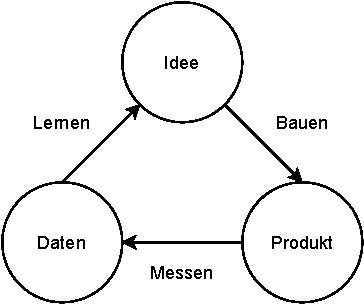
\includegraphics[width=0.5\columnwidth]{figures/lean-startup.pdf}
\caption{\label{fig:lean-startup}Iterationszyklus nach Lean Startup}
\end{figure}

Der Iterationszyklus ist in \autoref{fig:lean-startup} grafisch dargestellt\cite[vgl.][S. 75]{lean-startup}. Zunächst soll ein Produkt mit einer Idee starten. Diese Idee soll dann gebaut und anhand einer ausgewählten Metrik gemessen werden. Die Daten werden dann verwendet, um weitere Ideen zu generieren oder falsche Annahmen zu verwerfen. In dieser Arbeit wurden bereits mehrere Iterationszyklen durchlaufen, welche im Folgenden vorgestellt werden. \\

Zunächst ist die Idee entstanden, ein neues Rollenspiel in Anlehnung an Digimon World zu gestalten. Diese Idee wurde anhand von Interviews näher untersucht. Die daraus gewonnen Daten wurden analysiert und es sind neue Hypothesen aufgestellt worden. Dadurch ist die erste Iteration beendet worden. Die zweite Iteration startete mit den neu gewonnen Hypothesen. Eine Umfrage ist erstellt worden, welche erneut Daten generiert. In diesem Zyklus wurden Hypothesen belegt, aber einige auch widerlegt. Die quantitativen und qualitativen Daten wurden mit R untersucht und neue Erkenntnisse wurden geschlossen. Diese sind im dritten Iterationszyklus als Wireframes umgesetzt, welche mit unterschiedlichen Personen besprochen wurden. Während dieser Phase sind weitere Iterationszyklen im Bauen-Messen-Lernen-Zyklus entstanden, welche hier allerdings nicht näher erläutert werden. Im letzten Schritt wurden die gesammelten Daten zusammengetragen, um ein \ac{MVP} in der Godot Engine zu implementieren. Diese Daten müssen allerdings mit einer entsprechenden Metrik gemessen werden. \\

Für die Messung wird die Methode der schnellen iterativen Tests und Auswertungen(\ac{RITE}) verwendet\cite{rite-method}.
Die \ac{RITE}-Methode beschreibt ein Vorgehen, bei dem Testpersonen das Produkt testen und Probleme notiert werden. Diese werden in Form von Problemgruppen kategorisiert, welche sofort gelöst werden können, nach einiger Zeit gelöst werden können oder mehr Daten benötigt werden. In dieser Arbeit werden nur Probleme der ersten Kategorie abgehandelt. Alle weiteren Probleme werden nach der Arbeit bearbeitet. Getestet wird das \ac{MVP} von allen am Interview teilgenommenen Personen und dabei werden Probleme notiert. Diese Probleme sind im Repository als Issues in einer Kanban-Tafel aufgelistet.\\ 

\begin{figure}[H]
\centering
\begin{tikzpicture}
\begin{axis}[
    axis lines=middle,
    xmin=0, xmax=3,
    ymin=0, ymax=5,
    xtick={0, 1, 2, 3},
    ytick={1, 2, 3, 4, 5},
    x label style={at={(axis description cs:0.5,-0.1)},anchor=north},
    y label style={at={(axis description cs:-0.1,.5)},rotate=90,anchor=south},
    xlabel={Versuchsnummer},
    ylabel={Neu entdeckte Fehler},
    hide obscured x ticks=false,
    enlarge x limits={abs=10pt,upper},
    enlarge y limits={abs=10pt,upper},
]
\addplot [only marks, mark=o, mark options={blue,scale=2}] table {
1 5
2 4
3 2
};
\end{axis}
\end{tikzpicture}
\caption{\label{fig:rite-testing}Entdeckte Fehler im Testing}
\end{figure}

Nach jeder Testphase werden die Probleme zunächst gelöst, bevor die nächste Person die Testphase durchläuft. Auf diese Art und Weise können Lösungen bereits in der nächsten Testphase validiert werden und fallen nicht mehrfach auf. Alle, bis auf einen, Fehler in \autoref{fig:rite-testing} sind als Fehler der Stufe eins kategorisiert. Die Ausnahme bildet hierbei ein Fehler, welcher im ersten Versuch aufgefallen ist. Dieser konnte bis zum Versuch Nummer zwei nicht behoben werden und ist deswegen als Stufe zwei Fehler kategorisiert worden. Alle weiteren Fehler sind behoben worden. Es ist deutlich erkennbar, dass die erkannten Fehler für jeden weiteren Versuch abnehmen. Während jeder Testphase entstanden weitere Gespräche mit den Versuchspersonen und es wurde die Frage gestellt, ob die fertige Implementierung die Probleme der einzelnen Teilnehmenden lösen kann. Diese Frage wurde von allen teilnehmenden Personen bejaht.